\documentclass[12pt]{article}
\usepackage{light, graphicx}

\showsolutions
%\hidesolutions

\begin{document}

\recitation{3}{September 12, 2014}

%%%%%%%%%%%%%%%%%%%%%%%%%%%%%%%%%%%%%%%%%%%%%%%%%%%%%%%%%%%%%%%%%%%%%%%%%%%%%%%

%\insolutions{
%\section{State Machines}

%Recall from Lecture 3 (9/11) that an {\em invariant} is a property of
%a system (in lecture, that system was the 8-puzzle) that does not
%change, regardless of the system's behavior. Now we'll take a look at
%how we can make use of an important modeling tool --- a state machine
%--- to analyze systems. We'll see that finding invariants of state
%machines can often help us prove propositions.

%A {\em state machine} is an abstract model of a step-by-step
%process. The model consists of a collection of {\em states} and {\em
%transitions} between those states. More formally, we can define a
%state machine as

%\begin{itemize}
%\item a set of states: $Q$
%\item a designated start state: $q_0\in Q$
%\item a set of allowed transitions between states: $\delta\subseteq
%Q\times Q$.
%\end{itemize}
 
%\subsection{Example: Bounded Counter}

%Take, for example, a bounded counter that counts from 0 to 99 and
%overflows at 100. A diagram representing the corresponding state
%machine was shown in recitation. Note that in this example,
%there is a finite number of states. However, in general, the set of
%states might be infinite.

%this figure is incorrect (the counter one)
%% \begin{figure}
%% \begin{center}
%% 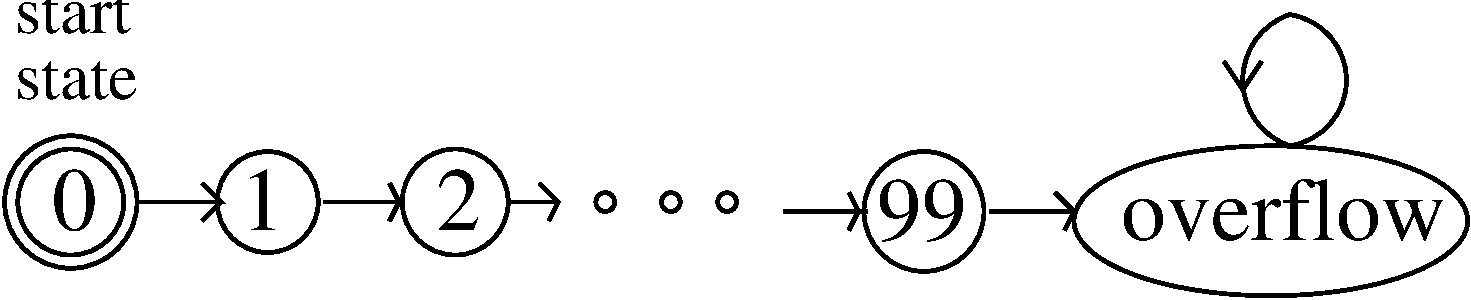
\includegraphics[scale = 0.6, trim = 0in 9in 0in 0in, clip]{counter}
%% \end{center}
%% \caption{State machine for the bounded counter example. In the figure,
%% the state labeled 0 is the start state. The self loop in the overflow
%% state means that once the machine overflows, there is no way for it to
%% transition out of this state.}
%% \label{counter}
%% \end{figure}

%\subsection{Example: Unbounded Counter}

%An unbounded counter is similar to a bounded counter except that there
%is an infinite number of states and no overflow. See
%Figure~\ref{unbounded}.

%\begin{figure}
%\begin{center}
%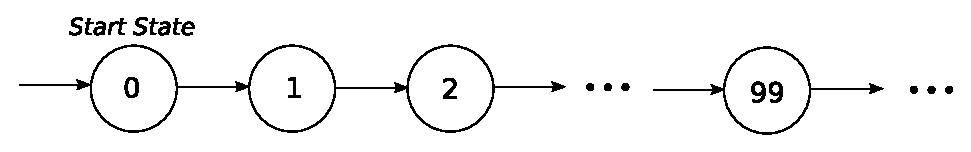
\includegraphics[scale = 0.6, trim = 0in 9in 0in 0in, clip]{unbounded}
%\end{center}
%\caption{State machine for the unbounded counter}
%\label{unbounded}
%\end{figure}
%}

%%%%%%%%%%%%%%%%%%%%%%%%%%%%%%%%%%%%%%%%%%%%%%%%%%%%%%%%%%%%%%%%%%%%%%%%%%%%%%%

\section{Problem: Breaking a chocolate bar}

We are given a chocolate bar with $m \times n$ squares of
chocolate, and our task is to divide it into $mn$ individual squares.  We
are only allowed to split one piece of chocolate at a time using a
vertical or a horizontal break.

For example, suppose that the chocolate bar is $2 \times 2$.  The
first split makes two pieces, both $2 \times 1$.  Each of these pieces
requires one more split to form single squares.  This gives a total of
three splits.

Prove that the number of times you split the bar does not depend on the sequence of splits you make.

\solution{

As with the ``stacking game'' from class, we approach the problem with experimentation, strong induction and a strong hypothesis. First we guess what the number of splits needed is:

\begin{theorem*}
To divide up a chocolate bar with $m \times n$ squares, we need at
most $m n - 1$ splits.
\end{theorem*}

This theorem does not immediately lend itself to an
  induction or strong induction proof, since there are {\it two} variables.  In general,
  propositions involving several natural-valued variables can often be
  proved by using a sort of nested induction  (make sure to try that).

However, in this case, we can get by with a single-variable induction and a trick.

Intuitively, to break up a big chocolate bar, we need one split to
make two pieces, and then we can break up the two pieces recursively.
This suggests a proof using strong induction on the {\em size} of the
chocolate bar, where size is measured in chocolate squares.  Now
instead of a problem involving two variables (the two dimensions), we
have a problem in one variable (the size).  With this simplification,
we can prove the theorem using strong induction.

\begin{proof}
The proof is by strong induction on the size of the chocolate bar.  Let
$P(k)$ be the proposition that a chocolate bar of size $k$ requires at
most $k - 1$ splits.  

\emph{Base case, $k=1$}: $P(1)$ is true because there is only a single
square of chocolate, and $1 - 1 = 0$ splits are required.

\emph{Induction step}: We suppose $k \geq 1$ and any chocolate bar of size
$s$, where $1 \leq s \leq k$, requires at most $s-1$ splits.  We must now
show there is a way to split a chocolate bar of size $k+1$ with at most
$k$ splits.

To do this, first break the chocolate bar of size $k+1$ into two smaller
pieces of size $p$ and $q$ where $p + q = k + 1$.  This is certainly
possible because the size of the bar is at least two.  Now the pieces of
sizes $p$ and $q$ are between one and $k$, so by strong induction,
breaking these two pieces into single squares requires only $p - 1$ and $q
- 1$ splits, respectively.  The total number of splits required to break
the bar of size $k+1$ into single squares is therefore at most $1 + (p -
1) + (q - 1) = p + q - 1 = (k + 1) - 1 = k$.

This shows that $P(k)$ implies $P(k+1)$, and the claim is proved by
strong induction.
\end{proof}
}

\newpage
\section{Problem: The Temple of Forever}

Each monk entering the Temple of Forever is given a bowl with 15 red
beads and 12 green beads.  Each time the Gong of Time rings, a monk
must do one of two things:

\begin{enumerate}

\item {\em Exchange}: If he has at least 3 red beads in his bowl, then he may exchange 3
red beads for 2 green beads.

\item {\em Swap}: He may replace each green bead in his bowl with a red bead and
replace each red bead in his bowl with a green bead.
That is, if he starts with $i$ red beads and $j$ green beads, then after he
performs this operation, he will have $j$ red beads and $i$ green beads.

\end{enumerate}

\noindent A monk may leave the Temple of Forever only when he has
exactly 5 red beads and 5 green beads in his bowl.

Let's look at how we can represent this problem as a state machine.

\begin{itemize}

\item 
What do the states of the machine look like? 
\solution{We can use variables such as $r$ to represent the number of
red beads and $g$ to represent the number of green beads. Then the
states can be represented as pairs $(r,g)$ for $r\geq 0, g\geq 0$.}

\item
Use the notation you developed above to represent the allowable
transitions in the state machine.

\solution{There are two possible transitions:
\begin{enumerate}
\item trade 3 red for 2 green ({\em exchange}): $(r,g)\rightarrow (r-3,g+2), r\geq 3$
\item swap red and green ({\em swap}): $(r,g)\rightarrow (g,r)$
\end{enumerate}
}

\item Expand the state machine diagram to the first three or four
  levels. Label the transitions according to the operation type (E for
  {\em exchange} or S for {\em swap}).

\solution{
You can see the diagram in Figure~\ref{solution}.


\begin{figure}
\begin{center}
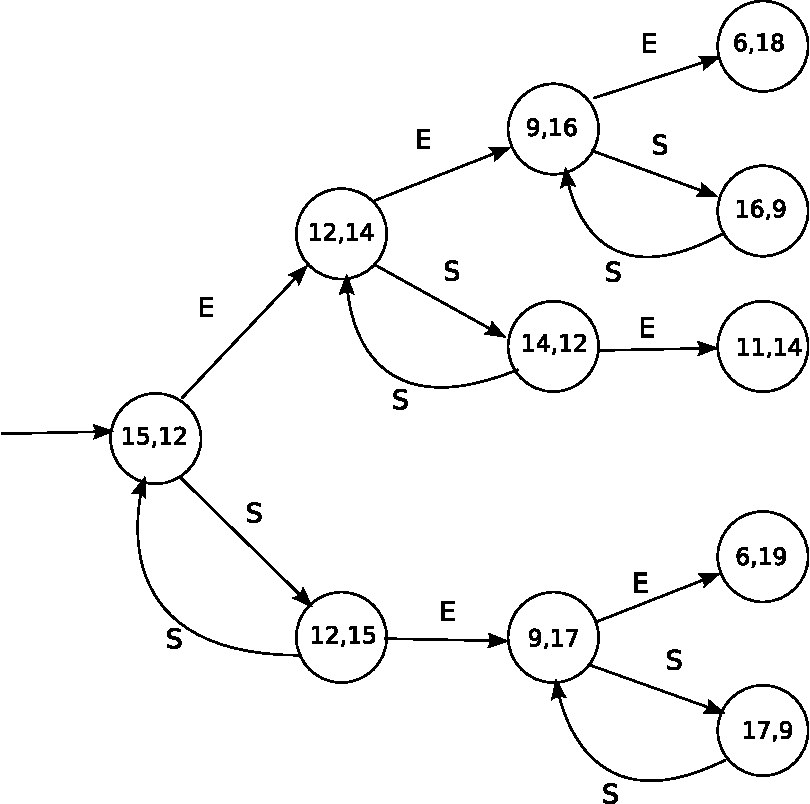
\includegraphics[scale = 0.6, trim = 0in 2in 1in 0in, clip]{diagram}
\caption{State machine diagram for first few levels}
\end{center}
\label{solution}
\end{figure}
}

\end{itemize}

\insolutions{

\subsection{Invariants and State Machines}

The Temple of Forever machine models every possible way of exchanging
beads at each time step according to the rules. We would like to know
whether the machine ever reaches the state $(5,5)$. By starting at the
start state and following the transition arrows through the state
diagram, we can trace the possible paths, or {\em executions}, of the
machine. So another way of stating our question is whether the state
we are interested in appears in some execution of the machine. If so,
then we can say that that state is {\em reachable}.

\begin{definition}
A state is called {\em reachable} if there is a path to it starting
from the start state, that is, if it appears in some execution.
\end{definition}

A useful technique for analyzing reachability is the identification of
{\em invariants} of the machine. An invariant will hold for all
reachable states of the machine. More formally,

\begin{definition}
  An {\em invariant} for a state machine is a predicate $P$ on state
  machines such that $P(q_0)$ holds (where $q_0$ is the start state of
  the machine), and whenever $P(q)$ is true of a state $q$, and
  $q\rightarrow r$ for some state $r$, then $P(r)$ holds.
\end{definition}

Since, by definition, an invariant holds for the start state and for
all transitions of the state machine, then we know (by induction) that
the invariant must hold for all reachable states. Therefore, if we
know some property to be an invariant, and we know that a certain
state violates that property, then we can say that this state is
unreachable.

} % end insolutions

Now we'll show that no monk can ever escape the Temple of Forever
because the state $(5,5)$ violates an invariant of the Temple of
Forever machine.

\begin{theorem}
No one ever leaves the Temple of Forever.
\end{theorem}

Prove this theorem by induction.  Begin by searching for an invariant
that holds initially and is maintained by each operation, but would be
violated by the condition required for departure.

\solution{
\begin{proof}
We use induction on the number of gong rings.  Let $P(n)$ be the
proposition that after $n$ rings, the number of red beads in the
monk's bowl minus the number of green beads is equal to $5k+2$ or
$5k+3$ for some integer $k$.

\noindent \textit{Base case:} $P(0)$ is true because initially (after
zero rings) the number of red beads minus the number of green beads is
$15 - 12 = 5 \cdot 0 + 3$.

\noindent \textit{Inductive step:} Now assume that $P(n)$ holds after
$n$ gong rings, where $n \geq 0$.  Let $r$ denote the number of red
beads in the monk's bowl, and let $g$ denote the number of green
beads.  In these terms, we are assuming that $r - g$ is equal to $5k +
2$ or $5k + 3$ for some integer $k$.  After $n + 1$ gong rings, there
are two cases to consider, depending on the monk's action:

\begin{enumerate}

\item If $r \geq 3$, then the monk may have exchanged 3 red beads for
2 green beads.  Thus, the number of red beads minus the number of
green becomes:
%
\[
(r - 3) - (g + 2) = (r - g) - 5
\]
%
This is equal to either $5 (k - 1) + 2$ or $5 (k - 1) + 3$, so
$P(n+1)$ is true.

\item Alternatively, the monk may have swapped every red bead for a
green bead and vice versa.  In this case, the number of reds minus the
number of greens becomes $g - r$.  If $r - g = 5k + 3$, then $g - r =
5 (-k) - 3 = 5 (-k-1) + 2$.  If $r - g = 5k + 2$, then $g - r = 5 (-k)
- 2 = 5 (-k-1) + 3$.  Thus, $P(n+1)$ is again true.

\end{enumerate}

Therefore, $P(n)$ implies $P(n+1)$ for all $n \geq 0$.

By the induction principle, $P(n)$ is true for all $n \geq 0$.  Since
the number of red beads minus the number of greens is always of the
form $5k+2$ or $5k+3$ and the difference required to leave the temple
does not match either form, no monk can ever leave the Temple of
Forever.
\end{proof}
}

Now let's take a look at a different property of the Temple of Forever
machine.

\begin{theorem}
  There is a finite number of reachable states in the Temple of
  Forever machine.
\end{theorem}

Prove this theorem. (Hint: First find an invariant that suggests an
upper bound on the number of reachable states. Be sure to prove the
invariant.)

\solution{ 

  We begin by noting that the Temple of Forever machine exhibits the
  following invariant:

\begin{lemma}\label{rgsum}
  For all reachable states, the total number of red beads and green
  beads in the monk's bowl --- $r+g$ --- is at most 27.
\end{lemma}

\begin{proof}
  We use induction on the number of gong rings.  Let $P(n)$ be the
  proposition that after $n$ gong rings, $r+g\leq 27$.

\noindent \textit{Base case:} $P(0)$ is true because initially (after
zero rings) the number of red beads plus the number of green beads is
$15 + 12 = 27$.

\noindent \textit{Inductive step:} Now assume that $P(n)$ holds after
$n$ gong rings, where $n \geq 0$.  Let $r$ denote the number of red
beads in the monk's bowl, and let $g$ denote the number of green
beads.  In these terms, we are assuming that $r + g$ is at most 27
after $n$ gong rings.  After $n + 1$ gong rings, there are two cases
to consider, depending on the monk's action:

\begin{enumerate}

\item If $r \geq 3$, then the monk may have exchanged 3 red beads for
2 green beads.  Thus, the number of red beads plus the number of
green becomes:
%
\[
(r - 3) + (g + 2) = (r + g) - 1
\]
%
Since, by the inductive hypothesis, $r+g\leq 27$, it follows that
$(r+g)-1\leq 27$, and so $P(n+1)$ is true.

\item Alternatively, the monk may have swapped every red bead for a
  green bead and vice versa.  In this case, the number of reds plus
  the number of greens becomes $g + r=r+g$. Thus, $P(n+1)$ is again
  true by the inductive hypothesis.

\end{enumerate}
\end{proof}

We now prove the theorem by showing that there is a finite upper bound
on the number of reachable states.

\begin{proof}
  We give a direct argument. Lemma~\ref{rgsum} tells us $r+g\leq 27$.
  This implies that there is an upper bound on the number of reachable
  states, since there can be at most 28 ways for $r$ and $g$ to sum to
  27, 27 ways to sum to 26, and so on.  Therefore, there can be at
  most $28+27+\ldots+1=\frac{29\cdot 28}{2}=406$ states in the Temple
  of Forever machine. Hence, there is a finite number of reachable
  states in the Temple of Forever machine.
\end{proof}

} % end solution

Inside the Temple of Forever, the Gong of Time rings on. As you may
well imagine, the monks begin to recognize that no matter how many
ways they try to exchange or swap their beads, they always seem to end
up in some state they've already been in before! For one or two monks,
this realization is all they need to propel them instantly into a
state of enlightenment. For the overwhelming majority, however, this
knowledge does nothing but weaken their resolve. They just get
depressed. Taking note of the mental state of this second group, the
Keeper of the Temple makes an unannounced appearance and proclaims to
the group, ``From now on, any monk who is able to visit 108 (108 being
the mystical number that encompasses all of existence\footnote{See
  http://astrologyforthesoul.com/vp/mysticalnumber108.html. Also
  consider: $42+24+42=108$.})  unique states will be allowed to leave
the Temple of Forever.''

Do the monks have any chance of leaving the Temple of Forever?

\begin{theorem}
  It is not possible to visit 108 unique states in the Temple of
  Forever machine.
\end{theorem}

Prove this theorem. (Hint: Consider a proof by contradiction.)

\solution{
\begin{proof}
  The proof is by contradiction. Assume that it {\em is} possible for
  a monk to visit 108 unique states in some execution of the Temple of
  Forever machine, and consider the sequence of moves that the monk
  must have made to visit these states. Each move in the sequence must
  be either an {\em exchange} or a {\em swap}, since these are the
  only legal moves. Now, whenever the monk performs an {\em exchange}
  operation, the sum $r+g$ decreases by one:
%
\[
(r - 3) + (g + 2) = (r + g) - 1
\]
%
In contrast, swaps do not have any effect on the sum. Furthermore, we
know that the sum $r+g$ must be at least 3 to perform an exchange
operation. Therefore, there can be at most 25 exchange operations in
the sequence.

Now consider swap operations: between each pair of exchanges in the
sequence, there may be an unlimited number of swaps. However, only a
single swap can take the monk to a new state: if at step $k$ the monk
is in state $(r,g)$, then at step $k+2$, he will return to the same
state. Therefore, an upper bound on the number of unique states in any
execution of the machine is $25+26+1=52$ (if swaps are inserted at
both the beginning and end of the sequence). But then this contradicts
the assumption that the monk visits 108 unique states, so no monk ever
leaves the Temple of Forever.

\end{proof}

} % end solution

What is the true maximal number of unique states a monk can visit in
any execution of the Temple of Forever machine? How can this number be
achieved?

\solution{ 

  The true maximum is 52. To achieve this number, the monk can perform
  sequential swaps and exchanges until he reaches the state $(5,2)$
  via an exchange. At this point, the longest path goes to $(2,4)$,
  via an exchange, instead of $(2,5)$, via a swap. This is because the
  path leading to $(2,5)$ ends at $(2,5)$, whereas the path leading to
  $(2,4)$ continues with swaps and exchanges, with the final state
  being $(2,0)$ (arrived at via a swap). However, the monk can reach
  52 unique states if, at state $(5,2)$, he performs two swap in a row
  to pick up state $(2,5)$. Alternatively, the monk can perform two
  swaps at the start state, picking up state $(12,15)$, and then
  continue with 25 pairs of sequential exchange, swap operations until
  he reaches $(2,0)$. This also generates a path with 52 unique states.

}

\end{document}
